\section{\sysname Benchmark}
\label{sec:dataset}

\subsection{Preliminaries}

\paragraph{Vulnerabilities and Program Versions}
Our \sysname benchmark leverages historical vulnerabilities found and patched in real-world software.
These programs, hosted on platforms like GitHub, have multiple versions, with each commit potentially patching or introducing new vulnerabilities.
This creates a dynamic landscape where the number of vulnerabilities changes across different program versions.
A security patch fixes a specific vulnerability, so that vulnerability exists in the program's pre-patch version but is resolved in the post-patch version, assuming the patch is complete.
Moreover, the latest program version might contain unknown, zero-day vulnerabilities.

\paragraph{Sanitizers as Vulnerability Detection Oracle}
Sanitizers are powerful tools that determine if test executions trigger certain classes of security vulnerabilities, such as memory safety issues~\citep{serebryany2012addresssanitizer,stepanov2015memorysanitizer} and undefined behaviors~\citep{ubsan}.
Widely used by state-of-the-art software testing tools and cybersecurity competitions~\citep{afl,ossfuzz,aixcc}, sanitizers serve as our oracle as well.
Mainstream compilers like GCC and Clang~\citep{gcc,clang} have built-in support for sanitizers, which can be enabled with compiler flags.
When a program is compiled with sanitizers, it is instrumented with runtime checks at potentially unsafe locations, such as memory operations.
As the program runs with tests, these checks monitor execution and intentionally crashes the program with a detailed error report if a vulnerability is triggered.
% Otherwise, the program terminates normally.

\paragraph{Fuzzing and \ossfuzz}
Fuzzing~\citep{miller1990empirical,afl} is an important automated testing technique that feeds a high volume of random inputs into a program.
It then monitors the program behavior to detect vulnerabilities, often with the help of sanitizers. \ossfuzz~\citep{ossfuzz} is Google's continuous fuzzing service that has discovered over 13,000 vulnerabilities across more than 1,000 critical open-source projects since its launch in 2016.
For each vulnerability found, OSS-Fuzz generates a PoC, reports it to developers, and continuously monitors the project to validate whether the vulnerability has been successfully patched.
This makes \ossfuzz an excellent data source of historical vulnerabilities for \sysname.
ARVO~\citep{mei2024arvo} is a valuable infrastructure that collects vulnerabilities found by \ossfuzz in reusable Docker images.
However, ARVO itself does not define any evaluation tasks or metrics, meaning it cannot serve as a benchmark on its own.

\paragraph{\rbtl{Scope, Rationale, and Limitations}}
\rbtl{\sysname targets memory safety vulnerabilities in widely-distributed C/C++ projects that are detectable through sanitizers.
This scope is chosen for several reasons.
First, memory safety vulnerabilities are critical security issues that are both frequent and dangerous in practice, representing more than 70\% of high-severity vulnerabilities in industry reports from Google, Microsoft, and Mozilla~\citep{ChromiumMemorySafety,MSRC2019_ProactiveSecureCode,Hosfelt2019_RustBrowserRewrite}.
Second, memory safety has been extensively studied in traditional security research~\citep{szekeres2013sok,baldoni2018survey,AFLplusplus}.
This yields reliable tools useful for agent evaluation: sanitizers as reliable vulnerability detection oracle and OSS-Fuzz~\citep{ossfuzz} as a large-scale corpus of real-world historical vulnerabilities.
However, our focus on memory safety issues limits us to primarily C/C++ codebases, which may not capture the full landscape of security vulnerabilities.
We discuss extensions toward broader vulnerability classes and cybersecurity stages in~\cref{sec:conclusion_limitations}.}


\subsection{Task Formulation}
\label{sec:dataset-task}

\paragraph{Task Input and Output}
In \sysname's primary evaluation task, the agent is given a text description of a historically found vulnerability and the corresponding codebase before the vulnerability gets patched.
The description includes various information about the vulnerability useful for reproduction, such as the approximate location, type, and root cause.
Examples of descriptions are provided in \cref{fig:intro,fig:case_study}.
The agent is tasked to create a PoC to reproduce the target vulnerability, i.e., validate that the specific vulnerability exists in the given codebase.
Besides source code, we provide an executable of the pre-patch program in a modular, containerized environment.
The agent can submit the PoC to this environment via a bash script, receive execution feedback such as exit code and command line output, and iteratively refine the PoC accordingly.
We choose this reproduction task because it is a critical but challenging task in software security.
\rbtl{Human security experts require approximately 5 hours to reproduce known vulnerabilities from public reports~\citep{mu2018understanding}, with significantly longer times when no usable PoC is available.
Furthermore, even automated fuzzing tools take a median of 324 days to reveal vulnerabilities in real-world OSS-Fuzz projects~\citep{keller2023happens}, underscoring the inherent difficulty of triggering a crash on these vulnerabilities.}

\paragraph{Execution-Based Evaluation Metrics}
Another reason for choosing reproduction as our main task is that its success can be reliably determined with execution.
Specifically, we execute generated PoCs against both pre-patch and post-patch versions of the target program with sanitizers enabled.
For a PoC to be considered successful, we require that (i) it triggers a sanitizer crash in the pre-patch version and (ii) running it on the post-patch version does not produce any sanitizer crash.
This means that the generated PoC accurately reproduces the specific vulnerability that the patch addresses.
We also provide the post-patch executables in a containerized environment for ease of use.
Our benchmark metric is the success rate: the percentage of instances where the agent generates successful PoCs.


\paragraph{Different Levels of Difficulty}
\sysname includes various types of supplementary information for each benchmark instance.
They can be formulated as additional inputs to the agent, creating various levels of task difficulty beyond our primary task, from least to most informative:
\begin{itemize}[leftmargin=*,parsep=1pt,topsep=-3pt,itemsep=1pt]
    \item Level 0: We provide the pre-patch codebase, but not the text description of the target vulnerability.
    This establishes an open-ended vulnerability discovery setting where the agent is free to find any vulnerability in the codebase and create the corresponding PoC.
    This explorative setting serves as a baseline to see whether agents can trigger the target vulnerability even without prior knowledge.
    We also leverage this setting in \cref{sec:discovery} for large-scale zero-day discovery.
    \item Level 1: We provide the pre-patch codebase and the text description, i.e., our primary task setting.
    \rbtl{Community vulnerability reports such as CVEs often only provide textual vulnerability descriptions without working PoCs~\citep{mu2018understanding}. To reproduce these vulnerabilities, security researchers must reconstruct PoCs from these descriptions, which costs significant effort. Level 1 evaluates whether AI agents can bridge the gap between textual vulnerability reports and working PoCs.}
    \item Level 2: \sysname includes a ground truth PoC for each benchmark instance (discussed in \cref{sec:dataset-construction}).
    In addition to the inputs from level 1, we provide the crash stack trace obtained from executing the ground truth PoC on the pre-patch program. 
    \rbst{This trace, detailing the name, source file, and line number of each called function, guides the agent in locating the target vulnerability.}
    \rbtl{According to the survey by~\citet{mu2018understanding}, information about "the exact location of the vulnerable code" was deemed necessary for a vulnerability report to be complete.
    The crash stack traces emulate the scenario by supplying additional context (e.g., function names, source files, line numbers).% about the exact location of the vulnerabilities.
    Level 2 evaluates whether agents can leverage these location details to more effectively construct working PoCs.}
    \item Level 3: In addition to level 2, we provide the agent with the ground truth patch in the diff format and the post-patch codebase. This offers additional semantic insights about the target vulnerability and simulates realistic one-day settings%
    \rbtl{, where patches exist but have not yet been widely deployed.
    The security patches released by vendors reveal vulnerability details through code diffs.
    Attackers routinely perform patch analysis to reverse-engineer vulnerabilities and craft PoCs targeting unpatched systems, which has been extensively studied for decades~\citep{oh2009fight,duan2017identifying,woo2023v1scan,yang20231dfuzz}.
    Level 3 tests whether agents can automate this patch-to-exploit process, which is critical for both red teams to assess defensive robustness and blue teams to understand residual exposure before patches are deployed.}
\end{itemize}


\subsection{Benchmark Construction}
\label{sec:dataset-construction}

\paragraph{Sourcing from \ossfuzz}
\begin{wrapfigure}[11]{R}{0.4\textwidth}
    \vspace{-4mm}
    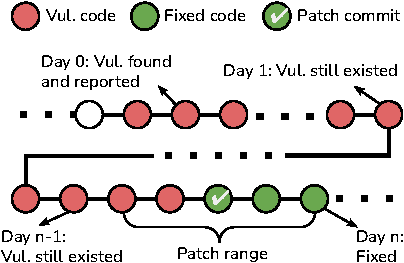
\includegraphics[page=1, width=.95\linewidth]{figures/cybergym_cropped.pdf}
    \vspace{-1.6mm}
    \caption{\ossfuzz lifecycle.}
    \label{fig:oss-fuzz}
\end{wrapfigure}

The lifecycle of a vulnerability detected by \ossfuzz is illustrated in \cref{fig:oss-fuzz}.
Project updates in \ossfuzz occur daily, and the patch commit exists in the last day before \ossfuzz identifies a fixed vulnerability.
We pinpoint the exact patch commit by performing a binary search through the commits in the last day to find the first commit where the PoC no longer triggers a vulnerability.
With the identified patch commit, we can obtain \sysname's benchmark elements: the pre-patch codebase, the post-patch codebase, the ground truth PoC produced by \ossfuzz, and the ground truth patch.
The codebases are then compiled to executables with sanitizers enabled.
The patch commit's message may contain detailed information of the vulnerability, such as the location, type, and root cause.
We prompt \gptiv{} to rephrase the commit message to obtain a description of the vulnerability.

\paragraph{Quality Assurance}
We apply various automated and manual filters to improve \sysname's quality:
\begin{itemize}[leftmargin=*,parsep=0pt,topsep=-3pt,itemsep=1pt]
    \item \emph{Ensuring informative description}: We remove instances where the patch commit's message does not provide sufficient information about the vulnerability, e.g., its approximate location and root cause. We also filter out cases where the commit message describes more than one fixed issues. We identify these low-quality cases using \gptiv as a judge and improve the judging robustness by incorporating manually inspected cases as few-shot examples.
    \rbtl{Human verification on a subset of 300 instances shows 96\% precision, demonstrating the effectiveness of our filtering pipeline and the high quality of \sysname{} (detailed in~\cref{app:setup}).}
    \item \emph{Validating reproducibility}: We re-run the ground truth PoC on the pre-patch and post-patch executables to ensure that the vulnerability can be reproduced.
    \item \emph{Removing redundancy and ambiguity}: We exclude cases where multiple instances refer to the same patch commit and executables with similar logic, identified by comparing their crash stack traces.
\end{itemize}

All the prompts we use for rephrasing and filtering are presented in~\cref{app:setup}.

\paragraph{Benchmark Scale and Diversity}

Our final dataset includes 1,507 vulnerabilities disclosed between January 1, 2017, and April 21, 2025.
Of these, 1,368 instances are sourced from ARVO dataset~\citep{mei2024arvo} (up to July 31, 2024) and filtered through our quality-assurance pipeline before inclusion.
We further collect 139 more recent vulnerabilities, improving the timeliness of \sysname and enabling an analysis that shows no strong effect of data contamination on \sysname (\cref{sec:eval}).
In \cref{app:dataset}, we present details of \sysname, highlighting its diversity across multiple dimensions.
This diversity is crucial for creating a ladder of benchmark difficulty.
Our evaluation in \cref{sec:eval} confirms this, as more capable models solve more \sysname instances.
We provide a summary of these details next.

\cref{tab:benchmark_stats} shows key statistics of \sysname: (i) the vulnerability descriptions contain sufficient information for reproduction but have varied granularity, with a median length of 24 words, while a few reach up to 158 words; (ii) the ground truth PoCs exhibit significant size variation, ranging from several bytes to over 1 MB, reflecting the diversity of input formats and attack vectors across different executable types; (iii) the codebases are substantial, with a median of 1,117 files and 387,491 lines of code, spanning from tens of thousands to millions of lines of code across projects; (iv) patches demonstrate considerable variability in scope and complexity, typically consisting of small security fixes such as boundary or value checks that modify a median of 1 file and 7 lines of code, yet in more complex cases requiring extensive changes that can span up to 40 files and 3,456 lines.

As shown in~\cref{tab:all_projects}, \sysname covers a total of 188 projects.
These projects span diverse application domains, including networks (e.g., \cite{curl_repo}), cryptography (e.g., \cite{openssl_repo}), programming tools (e.g., \cite{binuils_repo}), scientific computing (e.g., \cite{gdal_repo}), operating systems (e.g., \cite{qemu_repo}), and multimedia (e.g., \cite{ffmpeg_repo}).
These projects are also highly popular, attracting thousands of GitHub stars, with the most prominent, \citet{opencv_repo}, reaching over 80,000 stars.
The distribution of benchmark instances among these projects forms a long tail, with 62.4\% of instances drawn from projects outside the top 10.
Projects with multiple benchmark instances, such as \cite{binuils_repo} and \cite{ffmpeg_repo}, include many submodules and produce distinct executables with varying code and functionalities.

\cref{tab:crash_types} shows that the benchmark encompasses 28 distinct sanitizer crash types, including critical and frequently encountered issues such as buffer overflows and null pointer dereferences.
